
\pdfminorversion=4 % for acroread
%\documentclass[aspectratio=169,t,xcolor={usenames,dvipsnames}]{beamer}
\documentclass[aspectratio=169,t,handout,xcolor={usenames,dvipsnames}]{beamer}
\usepackage{../beamerstyle}
\usepackage{dsfont}
\usepackage{bm}
\usepackage[english]{babel}
\usepackage[utf8]{inputenc}
\usepackage{graphicx}
\usepackage{algorithm}
\usepackage[ruled,vlined,algo2e,linesnumbered]{algorithm2e}
%\usepackage[boxed,vlined]{algorithm2e}
\usepackage{hyperref}
\usepackage{booktabs}
\usepackage{mathtools}

\usepackage{amsmath,amssymb}
\usepackage{listings}
\lstset{frame=lines,framesep=3pt,numbers=left,numberblanklines=false,basicstyle=\ttfamily\small}

\usepackage{subfig}
\usepackage{multicol}
%\usepackage{appendixnumberbeamer}
%
\usepackage{tcolorbox}

\usepackage{pgfplots}
\usepackage{tikz}
\usetikzlibrary{trees} 
\usetikzlibrary{shapes.geometric}
\usetikzlibrary{positioning,shapes,shadows,arrows,calc,mindmap}
\usetikzlibrary{positioning,fadings,through}
\usetikzlibrary{decorations.pathreplacing}
\usetikzlibrary{intersections}
\usetikzlibrary{positioning,fit,calc,shadows,backgrounds}
\pgfdeclarelayer{background}
\pgfdeclarelayer{foreground}
\pgfsetlayers{background,main,foreground}
\tikzstyle{activity}=[rectangle, draw=black, rounded corners, text centered, text width=8em]
\tikzstyle{data}=[rectangle, draw=black, text centered, text width=8em]
\tikzstyle{myarrow}=[->, thick, draw=black]

% Define the layers to draw the diagram
\pgfdeclarelayer{background}
\pgfdeclarelayer{foreground}
\pgfsetlayers{background,main,foreground}

%\usepackage{listings}
%\lstset{numbers=left,
%  showstringspaces=false,
%  frame={tb},
%  captionpos=b,
%  lineskip=0pt,
%  basicstyle=\ttfamily,
%%  extendedchars=true,
%  stepnumber=1,
%  numberstyle=\small,
%  xleftmargin=1em,
%  breaklines
%}

 
\definecolor{blue}{RGB}{0, 74, 153}

\usetheme{Boadilla}
%\useinnertheme{rectangles}
\usecolortheme{whale}
\setbeamercolor{alerted text}{fg=blue}
\useoutertheme{infolines}
\setbeamertemplate{navigation symbols}{\vspace{-5pt}} % to lower the logo
\setbeamercolor{date in head/foot}{bg=white} % blue
\setbeamercolor{date in head/foot}{fg=white}
\setbeamercolor{author  in head/foot}{bg=white} %blue
\setbeamercolor{title in head/foot}{bg=white} % blue
\setbeamercolor{title}{fg=white, bg=blue}
\setbeamercolor{block title}{fg=white,bg=blue}
\setbeamercolor{block body}{bg=blue!10}
\setbeamercolor{frametitle}{fg=white, bg=blue}
\setbeamercovered{invisible}

\makeatletter
\setbeamertemplate{footline}
{
  \leavevmode%
  \hbox{%
  \begin{beamercolorbox}[wd=.333333\paperwidth,ht=2.25ex,dp=1ex,center]{author in head/foot}%
%    \usebeamerfont{author in head/foot}\insertshortauthor
  \end{beamercolorbox}%
  \begin{beamercolorbox}[wd=.333333\paperwidth,ht=2.25ex,dp=1ex,center]{title in head/foot}%
    \usebeamerfont{title in head/foot}\insertshorttitle
  \end{beamercolorbox}%
  \begin{beamercolorbox}[wd=.333333\paperwidth,ht=2.25ex,dp=1ex,right]{date in head/foot}%
    \usebeamerfont{date in head/foot}\insertshortdate{}\hspace*{2em}
%    \insertframenumber\hspace*{2ex} 
  \end{beamercolorbox}}%
  \vskip0pt%
}
\makeatother

%\pgfdeclareimage[height=1.2cm]{automl}{images/logos/automl.png}
%\pgfdeclareimage[height=1.2cm]{freiburg}{images/logos/freiburg}

%\logo{\pgfuseimage{freiburg}}

\renewcommand{\comment}[1]{
	\noindent
	%\vspace{0.25cm}
	{\color{red}{\textbf{TODO:} #1}}
	%\vspace{0.25cm}
}
\newcommand{\notefh}[1]{\textcolor{red}{\textbf{FH:} #1}}
\renewcommand{\comment}[1]{}
\newcommand{\hide}[1]{}
\newcommand{\cemph}[2]{\emph{\textcolor{#1}{#2}}}

\newcommand{\lit}[1]{{\footnotesize\color{black!60}[#1]}}

\newcommand{\litw}[1]{{\footnotesize\color{blue!20}[#1]}}


\newcommand{\myframe}[2]{\begin{frame}[c]{#1}#2\end{frame}}
\newcommand{\myframetop}[2]{\begin{frame}{#1}#2\end{frame}}
\newcommand{\myit}[1]{\begin{itemize}#1\end{itemize}}
\newcommand{\myblock}[2]{\begin{block}{#1}#2\end{block}}


\newcommand{\votepurple}[1]{\textcolor{Purple}{$\bigstar$}}
\newcommand{\voteyellow}[1]{\textcolor{Goldenrod}{$\bigstar$}}
\newcommand{\voteblue}[1]{\textcolor{RoyalBlue}{$\bigstar$}}
\newcommand{\votepink}[1]{\textcolor{Pink}{$\bigstar$}}

\newcommand{\diff}{\mathop{}\!\mathrm{d}}
\newcommand{\refstyle}[1]{{\small{\textcolor{gray}{#1}}}}
\newcommand{\hands}[0]{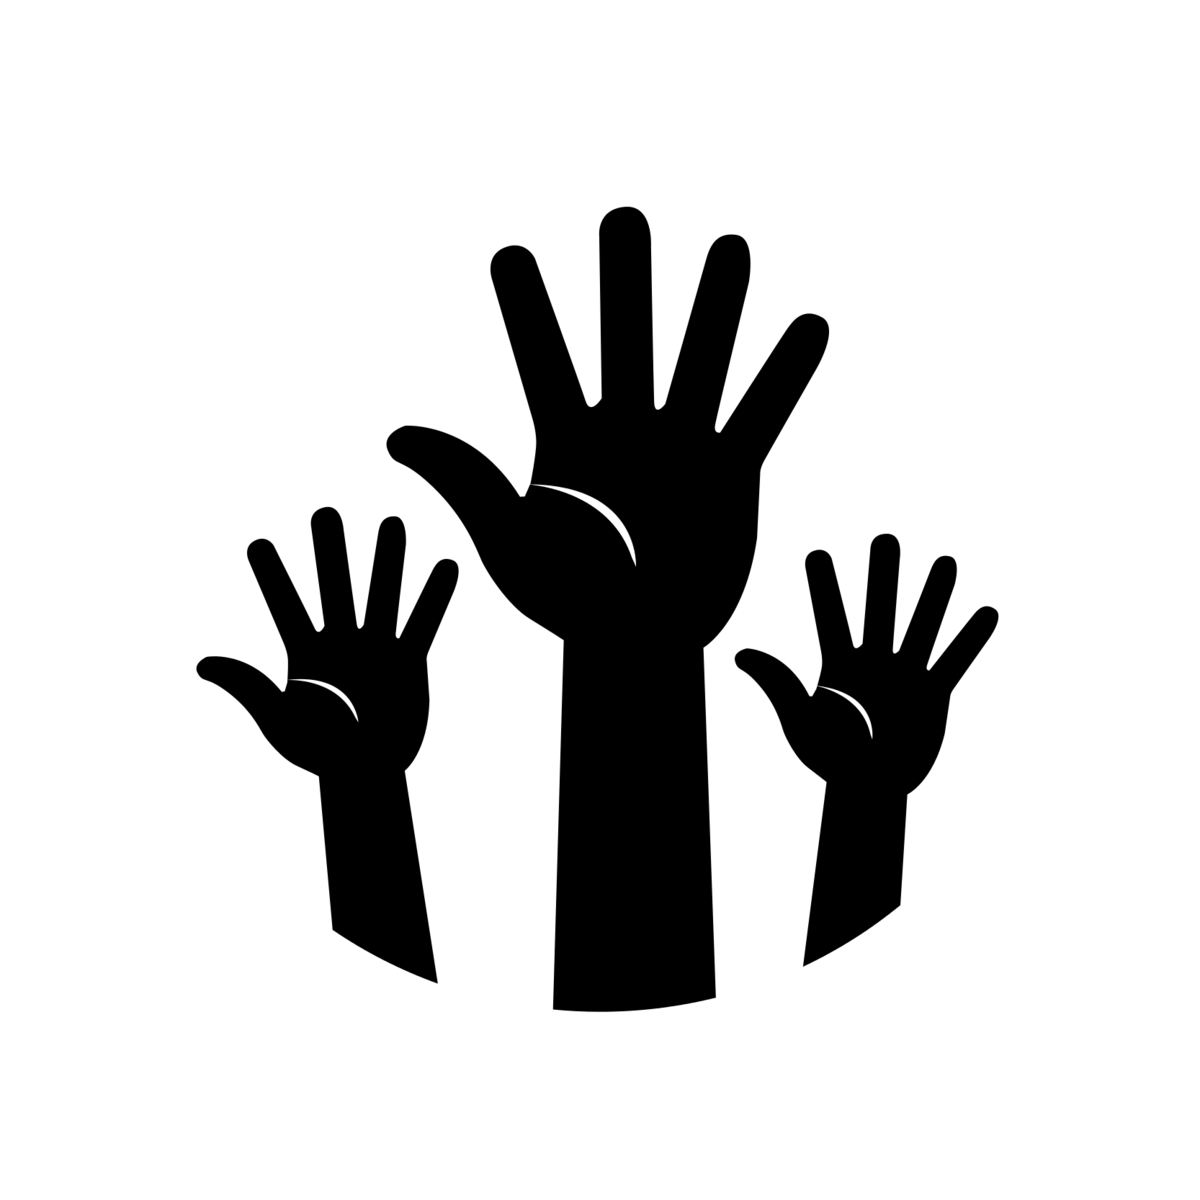
\includegraphics[height=1.5em]{images/hands}}
\newcommand{\transpose}[0]{{\textrm{\tiny{\sf{T}}}}}
\newcommand{\norm}{{\mathcal{N}}}
\newcommand{\cutoff}[0]{\kappa}
\newcommand{\instD}[0]{\dataset}
\newcommand{\insts}[0]{\mathcal{I}}
\newcommand{\inst}[0]{i}
\newcommand{\instI}[1]{i^{(#1)}}

% Iteration specific instance of variable/function/anything
% Introduced in the BO section, but moved up here to make it available within other macros
\newcommand{\iter}[2][\bocount]{{#2}^{(#1)}}

%--------HPO parameter macros-----------

% Parameter Configuration Space
\newcommand{\pcs}[0]{\pmb{\Lambda}}

% ???
\newcommand{\bx}[0]{\conf}

% Parameter Configuration
\newcommand{\conf}[0]{\pmb{\lambda}}

% Final Configuration
\newcommand{\finconf}[0]{\pmb{\hat{\lambda}}}

% Configuration corresponding to a given iteration -- better use \iter!
\newcommand{\confI}[1]{{\conf}^{(#1)}}

% Default Configuration
\newcommand{\defconf}[0]{{\conf}_{\text{def}}}

% Incumbent Configuration
\newcommand{\incumbent}[1][\bocount]{\iter[#1]{\finconf}}

% Optimal Configuration
\newcommand{\optconf}[0]{{\conf}^*}

% Configuration Space
\newcommand{\confs}[0]{\pcs}

%----------------------------------------

%\newcommand{\vlambda}[0]{\bm{\lambda}}
%\newcommand{\vLambda}[0]{\bm{\Lambda}}
\newcommand{\dataset}[0]{\mathcal{D}}
\newcommand{\datasets}[0]{\mathbf{D}}
\newcommand{\loss}[0]{L}
\newcommand{\risk}{\mathcal{R}}
\newcommand{\riske}{\mathcal{R}_{\text{emp}}}
\newcommand{\cost}[0]{c}
\newcommand{\costI}[1]{c^{(#1)}}

% Gaussian Process
\newcommand{\gp}{\mathcal{G}}
% Family of Objective Functions
\newcommand{\objF}{F}

%---------------BO Macros------------------

% BO loop counter
\newcommand{\bocount}{t}
% BO loop counter max, the counter runs from 1 to this value
\newcommand{\bobudget}{T}
% BO loop observation
\newcommand{\obs}[1][\conf]{\cost({#1})}
% BO loop observation space
\newcommand{\obsspace}{\mathcal{Y}}
% BO loop next observation
\newcommand{\bonextobs}{\obs[\iter{\conf}]}
% Acquisition Function, no args
\newcommand{\acq}{u}
% Standard Normal PDF
\newcommand{\pdf}{\phi}
% Standard Normal CDF
\newcommand{\cdf}{\Phi}
% Mean
\newcommand{\mean}{\mu}
% Standard Deviation
\newcommand{\stddev}{\sigma}
% Variance
\newcommand{\variance}{\sigma^2}
% Noise
\newcommand{\noise}{\nu}
% BO loop next selected sample
\newcommand{\bonextsample}{\confI{\bocount}}

% Single hyperparameter
\newcommand{\hyperparam}{\lambda}

% Single hyperparameter within a hyperparameter configuration
\newcommand{\hyperparami}[1][i]{{\hyperparam}_#1}

% Full definition of final configuration
\newcommand{\finconffull}{\incumbent[\bobudget]}

% Dataset
\newcommand{\datasetHPO}{{\dataset}_{HPO}}

% Dataset definition
\newcommand{\datasetHPOdef}{{\langle \bonextsample,\,\bonextobs \rangle}_{\bocount=1}^{\bobudget}}

% Double Display Fraction, forces large displays for everything in numerator and denominator
\newcommand\ddfrac[2]{\frac{\displaystyle #1}{\displaystyle #2}}

% Conditional Probability "Given That" Relation, source:https://tex.stackexchange.com/a/141685/205886
\newcommand\given[1][]{\:#1\vert\:}

% Expectation as a math operator
\DeclareMathOperator*{\E}{\mathbb{E}}

% Citation 
\newcommand{\source}[1]{
    \begin{flushright}
    	Source: \lit{#1}
    \end{flushright}
}
%-------------------------------------------

%Real numbers set
\newcommand{\realnum}{\mathbb{R}}
%Configuration space - do not use
%\newcommand{\configspace}{\Theta}
%Instances - do not use
%\newcommand{\instances}{\mathcal{I}}
%Expected value
\newcommand{\expectation}{\mathbb{E}}
%Kernel
\newcommand{\kernel}{\kappa}
%Constraint function
\newcommand{\constraintf}{c}
%Normal distribution
\newcommand{\normaldist}{\mathcal{N}}

% \renewcommand{\vec}[1]{\mathbf{#1}}
\newcommand{\hist}[0]{\dataset_{\text{Hist}}}
\newcommand{\param}[0]{p}
\newcommand{\algo}[0]{\mathcal{A}}
\newcommand{\algos}[0]{\mathbf{A}}
%\newcommand{\nn}[0]{N}
\newcommand{\feats}[0]{\mathcal{X}_{\text{meta}}}
\newcommand{\feat}[0]{\x_{\text{meta}}}
%\newcommand{\cluster}[0]{\vec{h}}
%\newcommand{\clusters}[0]{\vec{H}}
\newcommand{\perf}[0]{\mathbb{R}}
%\newcommand{\surro}[0]{\mathcal{S}}
\newcommand{\surro}[0]{\hat{\cost}}
\newcommand{\func}[0]{f}
\newcommand{\epm}[0]{\surro}
\newcommand{\portfolio}[0]{\mathbf{P}}
\newcommand{\schedule}[0]{\mathcal{S}}

% Machine Learning
\newcommand{\mdata}[0]{\dataset_{\text{meta}}}
\newcommand{\datasettrain}[0]{\dataset_{\text{train}}}
\newcommand{\datasetval}[0]{\dataset_{\text{val}}}
\newcommand{\datasettest}[0]{\dataset_{\text{test}}}
\newcommand{\x}[0]{\mathbf{x}}
\newcommand{\y}[0]{y}
\newcommand{\xI}[1]{\mathbf{x}^{(#1)}}
\newcommand{\yI}[1]{y^{(#1)}}
\newcommand{\fx}{f(\mathbf{x})}  % f(x), continuous prediction function
\newcommand{\Hspace}{\mathcal{H}} % hypothesis space where f is from
\newcommand{\fh}{\hat{f}}       % f hat, estimated prediction function

% Deep Learning
\newcommand{\weights}[0]{\theta}
\newcommand{\metaweights}[0]{\phi}


% reinforcement learning
\newcommand{\policies}[0]{\mathbf{\Pi}}
\newcommand{\policy}[0]{\pi}
\newcommand{\actionRL}[0]{a}
\newcommand{\stateRL}[0]{s}
\newcommand{\statesRL}[0]{\mathcal{S}}
\newcommand{\rewardRL}[0]{r}
\newcommand{\rewardfuncRL}[0]{\mathcal{R}}

\RestyleAlgo{algoruled}
\DontPrintSemicolon
\LinesNumbered
\SetAlgoVlined
\SetFuncSty{textsc}

\SetKwInOut{Input}{Input}
\SetKwInOut{Output}{Output}
\SetKw{Return}{return}

%\newcommand{\changed}[1]{{\color{red}#1}}

%\newcommand{\citeN}[1]{\citeauthor{#1}~(\citeyear{#1})}

\renewcommand{\vec}[1]{\mathbf{#1}}
\DeclareMathOperator*{\argmin}{arg\,min}
\DeclareMathOperator*{\argmax}{arg\,max}

%\newcommand{\aqme}{\textit{AQME}}
%\newcommand{\aslib}{\textit{ASlib}}
%\newcommand{\llama}{\textit{LLAMA}}
%\newcommand{\satzilla}{\textit{SATzilla}}
%\newcommand{\satzillaY}[1]{\textit{SATzilla'{#1}}}
%\newcommand{\snnap}{\textit{SNNAP}}
%\newcommand{\claspfolioTwo}{\textit{claspfolio~2}}
%\newcommand{\flexfolio}{\textit{FlexFolio}}
%\newcommand{\claspfolioOne}{\textit{claspfolio~1}}
%\newcommand{\isac}{\textit{ISAC}}
%\newcommand{\eisac}{\textit{EISAC}}
%\newcommand{\sss}{\textit{3S}}
%\newcommand{\sunny}{\textit{Sunny}}
%\newcommand{\ssspar}{\textit{3Spar}}
%\newcommand{\cshc}{\textit{CSHC}}
%\newcommand{\cshcpar}{\textit{CSHCpar}}
%\newcommand{\measp}{\textit{ME-ASP}}
%\newcommand{\aspeed}{\textit{aspeed}}
%\newcommand{\autofolio}{\textit{AutoFolio}}
%\newcommand{\cedalion}{\textit{Cedalion}}
\newcommand{\fanova}{\textit{fANOVA}}
\newcommand{\sbs}{\textit{SB}}
\newcommand{\oracle}{\textit{VBS}}

% like approaches
\newcommand{\claspfoliolike}[1]{\texttt{claspfolio-#1-like}}
\newcommand{\satzillalike}[1]{\texttt{SATzilla'#1-like}}
\newcommand{\isaclike}{\texttt{ISAC-like}}
\newcommand{\ssslike}{\texttt{3S-like}}
\newcommand{\measplike}{\texttt{ME-ASP-like}}

\newcommand{\irace}{\textit{I/F-race}}
\newcommand{\gga}{\textit{GGA}}
\newcommand{\smac}{\textit{SMAC}}
\newcommand{\paramils}{\textit{ParamILS}}
\newcommand{\spearmint}{\textit{Spearmint}}
\newcommand{\tpe}{\textit{TPE}}


\usepackage{pifont}
\newcommand{\itarrow}{\mbox{\Pisymbol{pzd}{229}}}
\newcommand{\ithook}{\mbox{\Pisymbol{pzd}{52}}}
\newcommand{\itcross}{\mbox{\Pisymbol{pzd}{56}}}
\newcommand{\ithand}{\mbox{\raisebox{-1pt}{\Pisymbol{pzd}{43}}}}

%\DeclareMathOperator*{\argmax}{arg\,max}

\newcommand{\ie}{{\it{}i.e.\/}}
\newcommand{\eg}{{\it{}e.g.\/}}
\newcommand{\cf}{{\it{}cf.\/}}
\newcommand{\wrt}{\mbox{w.r.t.}}
\newcommand{\vs}{{\it{}vs\/}}
\newcommand{\vsp}{{\it{}vs\/}}
\newcommand{\etc}{{\copyedit{etc.}}}
\newcommand{\etal}{{\it{}et al.\/}}

\newcommand{\pscProc}{{\bf procedure}}
\newcommand{\pscBegin}{{\bf begin}}
\newcommand{\pscEnd}{{\bf end}}
\newcommand{\pscEndIf}{{\bf endif}}
\newcommand{\pscFor}{{\bf for}}
\newcommand{\pscEach}{{\bf each}}
\newcommand{\pscThen}{{\bf then}}
\newcommand{\pscElse}{{\bf else}}
\newcommand{\pscWhile}{{\bf while}}
\newcommand{\pscIf}{{\bf if}}
\newcommand{\pscRepeat}{{\bf repeat}}
\newcommand{\pscUntil}{{\bf until}}
\newcommand{\pscWithProb}{{\bf with probability}}
\newcommand{\pscOtherwise}{{\bf otherwise}}
\newcommand{\pscDo}{{\bf do}}
\newcommand{\pscTo}{{\bf to}}
\newcommand{\pscOr}{{\bf or}}
\newcommand{\pscAnd}{{\bf and}}
\newcommand{\pscNot}{{\bf not}}
\newcommand{\pscFalse}{{\bf false}}
\newcommand{\pscEachElOf}{{\bf each element of}}
\newcommand{\pscReturn}{{\bf return}}

%\newcommand{\param}[1]{{\sl{}#1}}
\newcommand{\var}[1]{{\it{}#1}}
\newcommand{\cond}[1]{{\sf{}#1}}
%\newcommand{\state}[1]{{\sf{}#1}}
%\newcommand{\func}[1]{{\sl{}#1}}
\newcommand{\set}[1]{{\Bbb #1}}
%\newcommand{\inst}[1]{{\tt{}#1}}
\newcommand{\myurl}[1]{{\small\sf #1}}

\newcommand{\Nats}{{\Bbb N}}
\newcommand{\Reals}{{\Bbb R}}
\newcommand{\extset}[2]{\{#1 \; | \; #2\}}

\newcommand{\vbar}{$\,\;|$\hspace*{-1em}\raisebox{-0.3mm}{$\,\;\;|$}}
\newcommand{\vendbar}{\raisebox{+0.4mm}{$\,\;|$}}
\newcommand{\vend}{$\,\:\lfloor$}


\newcommand{\goleft}[2][.7]{\parbox[t]{#1\linewidth}{\strut\raggedright #2\strut}}
\newcommand{\rightimage}[2][.3]{\mbox{}\hfill\raisebox{1em-\height}[0pt][0pt]{\includegraphics[width=#1\linewidth]{#2}}\vspace*{-\baselineskip}}





%\newcommand{\a}[0]{\mathbf{a}}
%\newcommand{\y}[0]{\mathbf{y}}
\newcommand{\q}[0]{\mathbf{q}}
\newcommand{\Xspace}[0]{\mathcal{X}}
\newcommand{\inducer}{\mathcal{I}}

\title[AutoML: Overview]{Multi-criteria Optimization}
\subtitle{Practical Applications}
\author[Bernd Bischl]{\underline{Bernd Bischl} \and Frank Hutter \and Lars Kotthoff\newline \and Marius Lindauer \and Joaquin Vanschoren}
\institute{}
\date{}



% \AtBeginSection[] % Do nothing for \section*
% {
%   \begin{frame}{Outline}
%     \bigskip
%     \vfill
%     \tableofcontents[currentsection]
%   \end{frame}
% }

\begin{document}

	\maketitle

\begin{frame}[allowframebreaks]{Practical Applications in Machine Learning}

    \textbf{ROC Optimization}: Balance \emph{true positive} and \emph{false positive} rates
  \begin{itemize}
    \item Typically unbalanced classification tasks with unspecified costs.
    \item Many related measures, e.g., \emph{positive predicted value} or \emph{false discovery rate}, exist and can be of interest as well.
  \end{itemize}

\textbf{Efficient Models}:
    Balance \emph{predictive performance} with \emph{prediction time}, \emph{energy consumption} and/or \emph{model size}.
  \begin{itemize}
    \item Time: Models in production models need to predict fast.
    \item Size / Energy consumption: Models should be deployed on a mobile/edge device and not use much power.
  \end{itemize}

\textbf{Fair Models}:
  Balance \emph{predictive performance} and \emph{fairness}.
  \begin{itemize}
    \item Model has to be fair regarding subgroups in the data, e.g. gender.
    \item Many different approaches to quantify fairness exist.
  \end{itemize}

\end{frame}

\begin{frame}{ROC Optimization - Setup}

  Again, we want to train a \textit{spam detector} on the popular Spam dataset\footnote{\url{https://archive.ics.uci.edu/ml/datasets/spambase}}.

\begin{columns}
\begin{column}{0.5\textwidth}
\begin{itemize}
        \item Learning algorithm: SVM with RBF kernel.
        \item Hyperparameters to optimize: \\
        \begin{tabular}{rl}
        \texttt{cost} & $[2^{-15}, 2^{15}]$ \\
        $\gamma$ & $[2^{-15}, 2^{15}]$ \\
        Threshold $t$ & $[0,1]$ \\
        \end{tabular}
        \item Objective: \emph{minimize} false positive rate (FPR) and \emph{maximize} true positive rate (TPR), evaluated through 5-fold CV
\end{itemize}
\end{column}%
\begin{column}{0.5\textwidth}
\begin{itemize}
        \item Optimizer: Multi-criteria Bayesian optimization:
            \begin{itemize}
              \item ParEGO with $\rho = 0.05$, $s = 100000$.
              \item Acquisition function $\acq$: \emph{Confidence Bound} with $\alpha = 2$.
              \item Budget: $100$ evaluations
            \end{itemize}
        \item Tuning is conducted on a training holdout and all hyperparameters configurations of the Pareto front are validated on an outer validation set.
\end{itemize}
\end{column}
\end{columns}
\vspace{0.5cm}
{\footnotesize For simplicity we refrain from optimizing the threshold parameter independently posthoc.}
\end{frame}

\begin{frame}{ROC Optimization - Result I}

\begin{columns}
\begin{column}{0.45\textwidth}
  We notice here:
  \begin{itemize}
    \item Compared to the \emph{random search}: Many \emph{ParEGO} evaluations are on the estimated Pareto front.
    \item The Pareto front of \emph{ParEGO} dominates most points from the \emph{random search}.
    \item The dominated hypervolume to the reference point $(1,1)$ is:
    \begin{tabular}{rl}
    \emph{ParEGO:} & 0.965\\
    \emph{random search:} & 0.959\\
    \end{tabular}
  \end{itemize}
  Note: The Pareto front does not reflect the stochastic characteristic of our objective.
\end{column}%
\begin{column}{0.5\textwidth}
  \begin{figure}
  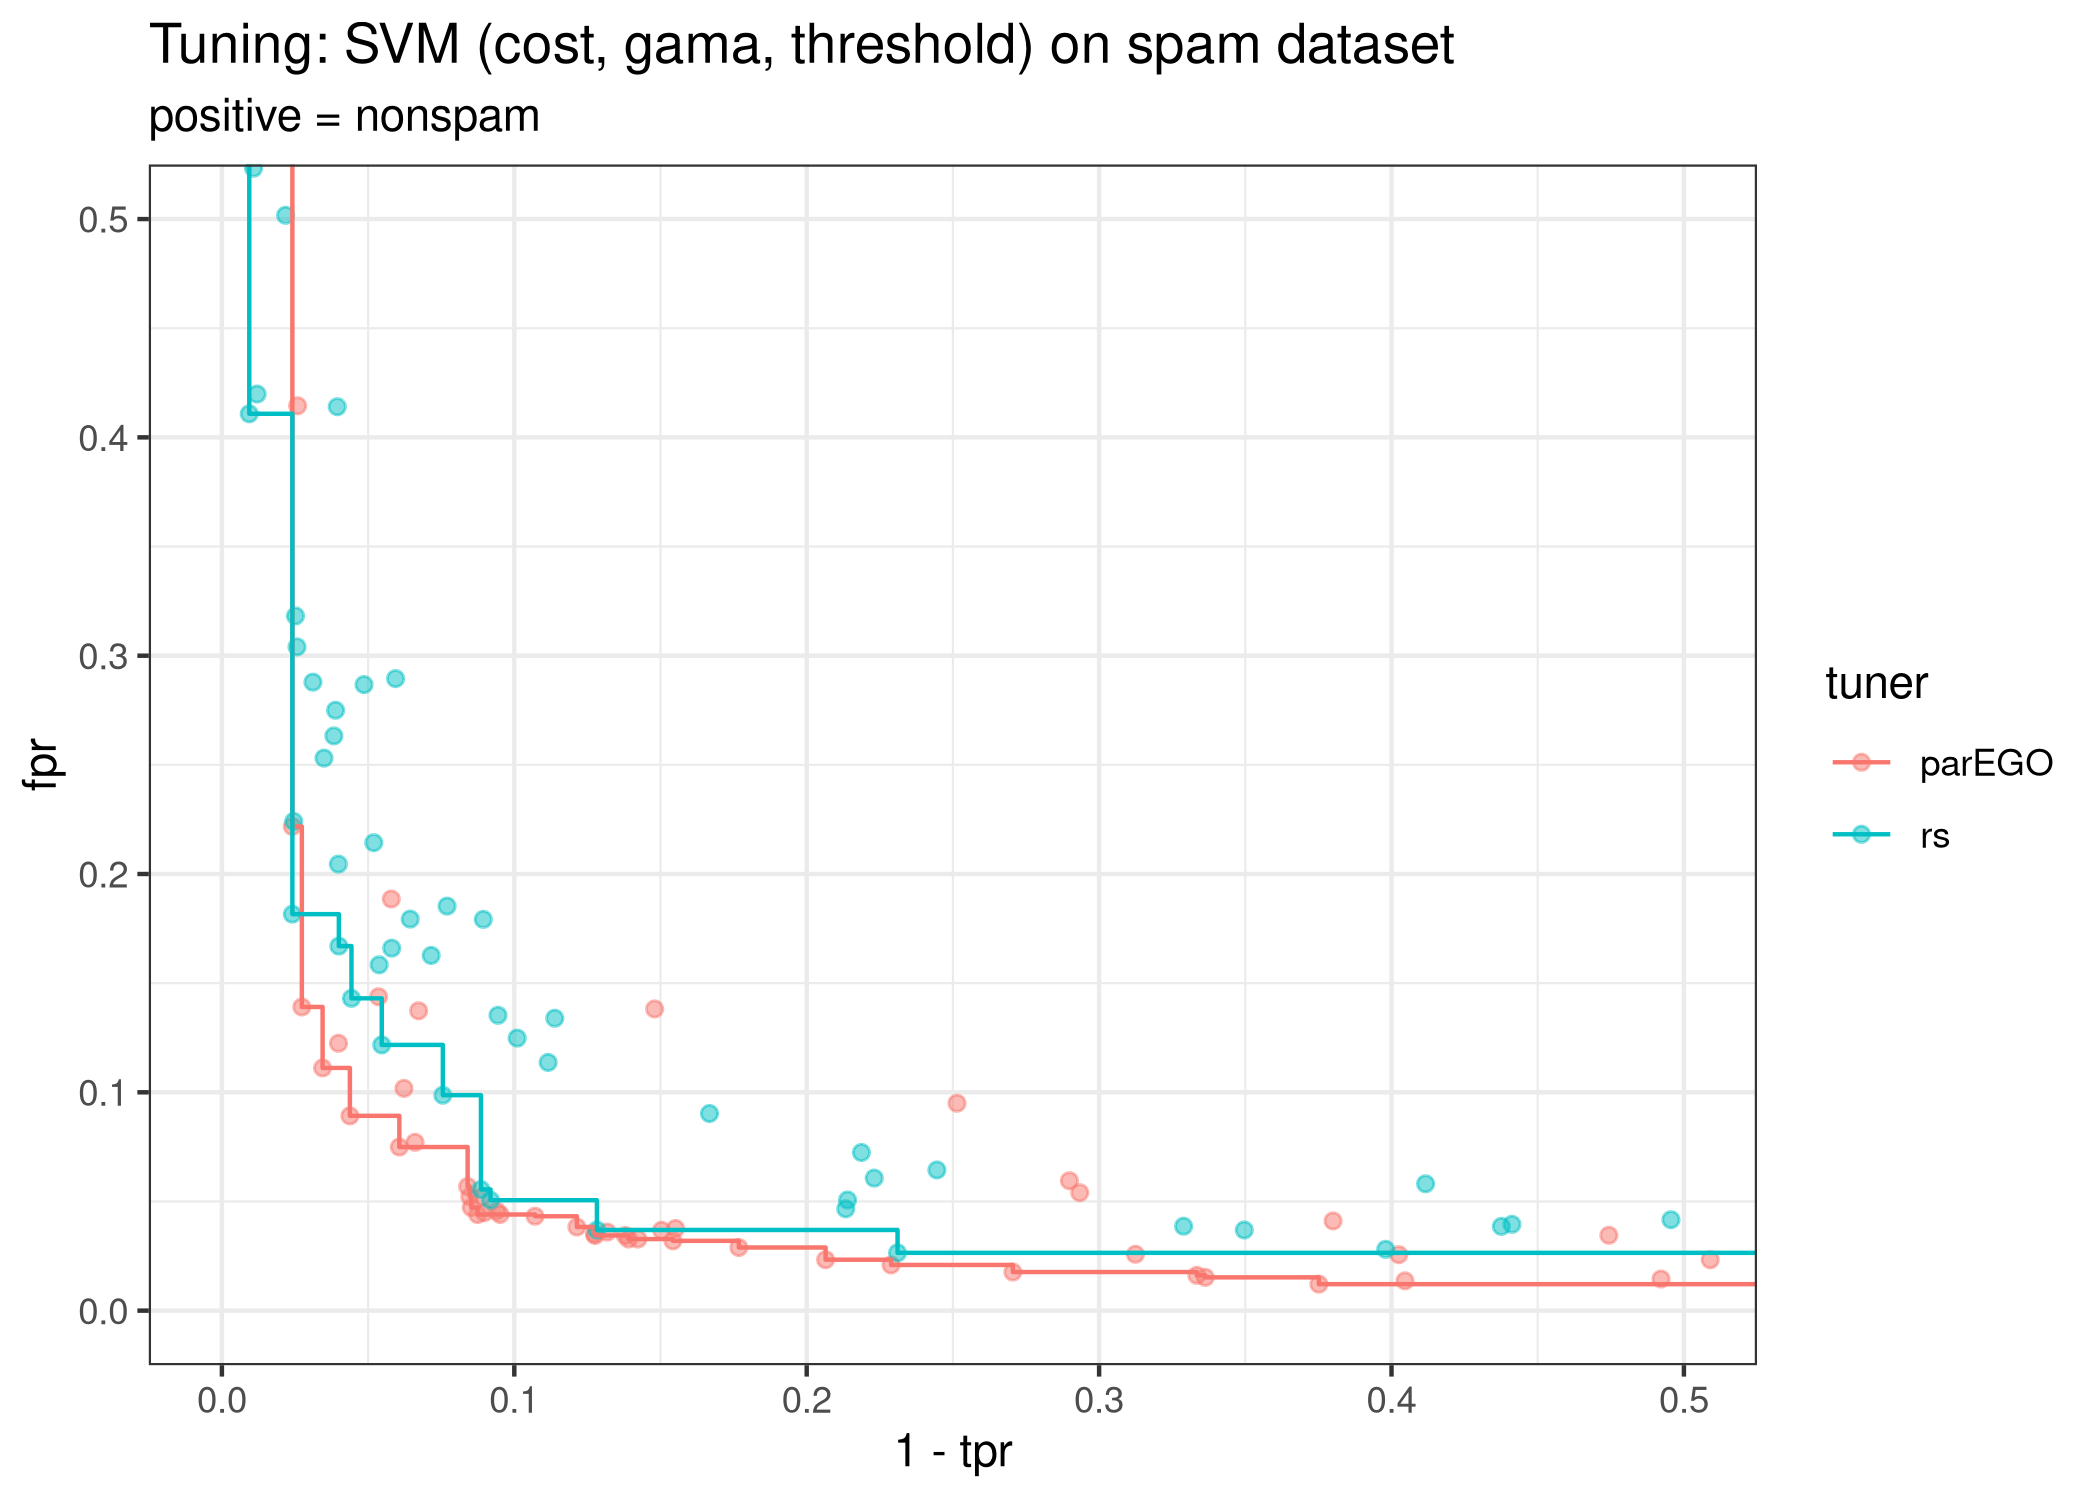
\includegraphics[width=\textwidth]{images/example_parego_spam.png}
  \end{figure}
\end{column}
\end{columns}

\end{frame}

\begin{frame}{ROC Optimization - Result II}

\begin{columns}
\begin{column}{0.45\textwidth}
  We validate the configurations on the Pareto front on a holdout:
  \begin{itemize}
    \item<1-> The performance on the validation set varies slightly.
    \item<1-> The TPR got slightly better but the FPR got slightly worse.
    \item<1-> On the validation set, some configurations get dominated by others.
    \item<2> The dominated hypervolume of the validation set is:
    \begin{tabular}{rl}
    \emph{ParEGO:} & 0.960\\
    \emph{random search:} & 0.961\\
    \end{tabular}
  \end{itemize}
\end{column}%
\begin{column}{0.5\textwidth}
  \begin{figure}
  \includegraphics<1>[width=\textwidth]{images/example_parego_spam_outer.png}
  \includegraphics<2>[width=\textwidth]{images/example_parego_spam_outer_pareto.png}
  \end{figure}
\end{column}
\end{columns}

\end{frame}

\begin{frame}{Efficient Models - Overview}

\begin{itemize}
  \item "Efficiency" can be:
  \begin{itemize}
    \item Memory consumption of the model
    \item Training or prediction time
    \item Number of features needed
    \item Energy consumption for prediction
    \item \ldots
  \end{itemize}
  \item Some hyperparameters have a strong impact on the efficiency of a model, e.g.,
  \begin{itemize}
    \item Number of trees in Random Forests or gradient tree boosting,
    \item Number, size and type of layers in neural networks,
    \item L1 regularization penalties,
    \item ...
  \end{itemize}
  \item Other hyperparameters can have no influence on efficiency.
  \item Optimizing over multiple algorithms of varying efficiency at the same time.
\end{itemize}

\end{frame}

\begin{frame}{Efficient Models - Example: Feature Selection I}

Goals of Feature Selection:
\begin{itemize}
  \item Identify an informative feature subset
  \item with only a small drop in predictive performance.
\end{itemize}
Problem Statement:
\[
\min_{\conf \in \pcs, s \in \{0,1\}^p}\left( \widehat{GE}\left(\inducer(\dataset, \conf, s)\right), \frac{1}{p}\sum_{i=1}^p s_i \right)
\] 
\begin{itemize}
  \item Problem: Feature selection and hyperparameter tuning are usually two separate steps. 
  \item Solution: Identify an informative subset of features and a good hyperparameter configuration \textbf{simultaneously}.

\end{itemize}
\begin{figure}
  \centering
  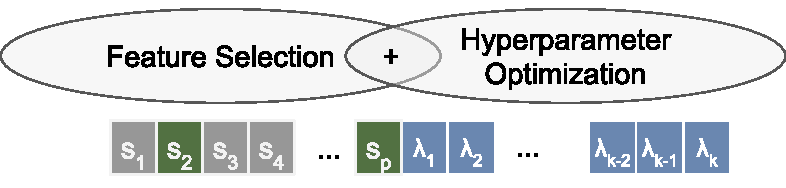
\includegraphics[width = 0.5\linewidth]{images/mosmafs_presentation_p14.pdf}
\end{figure}
    
\end{frame}

\begin{frame}{Efficient Models - Example: Feature Selection II}
Idea: \emph{Multi-Objective Hyperparameter Tuning and Feature Selection  using Filter Ensembles}\footnote{\url{https://arxiv.org/pdf/1912.12912.pdf}}:

  \begin{itemize}
    \item Pre-calculate multiple \emph{feature filter} values.
    
    \begin{figure}
      \centering
      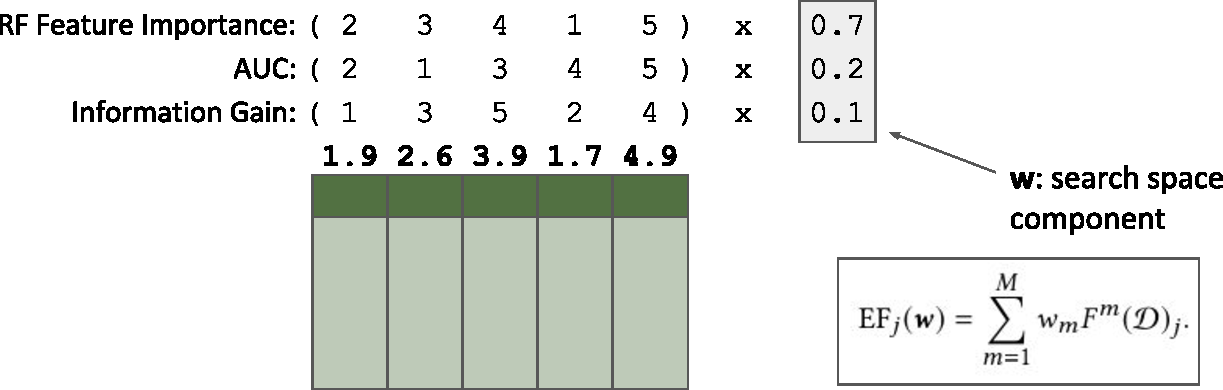
\includegraphics[width = 0.7\linewidth]{images/mosmafs_presentation_p39.pdf}
    \end{figure}

    \item New joint search space: $\pcs = \tilde{\pcs} \cup \{w_1, \ldots, w_p ,\tau \}$
    \begin{itemize}
      \item Hyperparameters of learner: $\tilde{\pcs}$
      \item Weight of each \emph{feature filter} value vector: $w_1, \ldots, w_p$
      \item Fraction of features to keep $\tau$
    \end{itemize}
    
  \end{itemize}  

\end{frame}

\begin{frame}{Efficient Models - Example: FLOPS}
Image Classification on CIFAR-10 dataset\footnote{\url{https://arxiv.org/pdf/1904.09035.pdf}}
  \begin{columns}
  \begin{column}{0.65\textwidth}
    \begin{itemize}
      \item Objective: \emph{accuracy} vs.\ \emph{FLOPS} (floating point operations, per observation)
      \item Learner: \emph{DenseNet-121} (Densely Connected Convolutional Networks)
      \item Search Space:\\
        \begin{tabular}{rl}
          \texttt{growth rate in all four blocks} ($k$) & $[8,32]$ \\ %growth rate: k_l = k_0 + k (l-1), how much information is added in each layer
          \texttt{layers in first block} & $[4, 6]$ \\
          \texttt{layers in second block} & $[4, 12] $ \\
          \texttt{layers in third block} & $[4, 24] $ \\
          \texttt{layers in fourth block} & $[4, 16] $ \\
        \end{tabular}
      \item Tuner: \emph{Particle Swarm Optimization}
    \end{itemize}
  \end{column}%
  \begin{column}{0.35\textwidth}
    \begin{figure}
    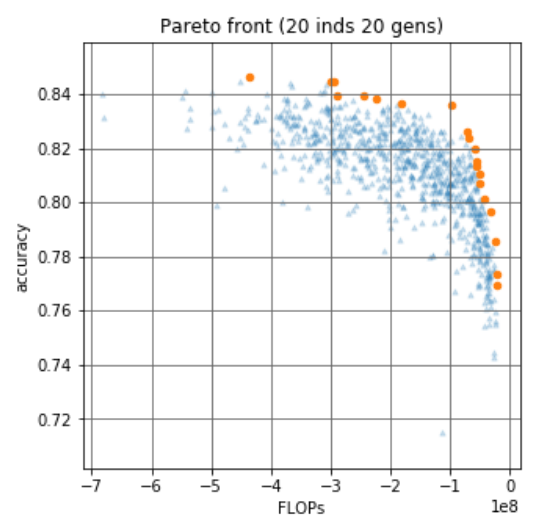
\includegraphics[width=\textwidth]{images/Wang_et_al_2019_Evolving_Deep_Neural_Networks_fig7_1.png}
    \end{figure}
  \end{column}
  \end{columns}


\end{frame}

\begin{frame}{Fair Models - The \texttt{Adult} dataset}
\begin{columns}
\begin{column}{0.4\textwidth}
Dataset: \texttt{Adult}
\begin{itemize}
  \footnotesize
  \item  Source: US Census database, 1994, \url{https://www.openml.org/d/1590}.
  \item 48842 observations
  \item Target: binary, income above 50k
  \item 14 features: \texttt{age, education, hours.per.week, marital.status, native.country, occupation, race, relationship, sex, \ldots}
\end{itemize}
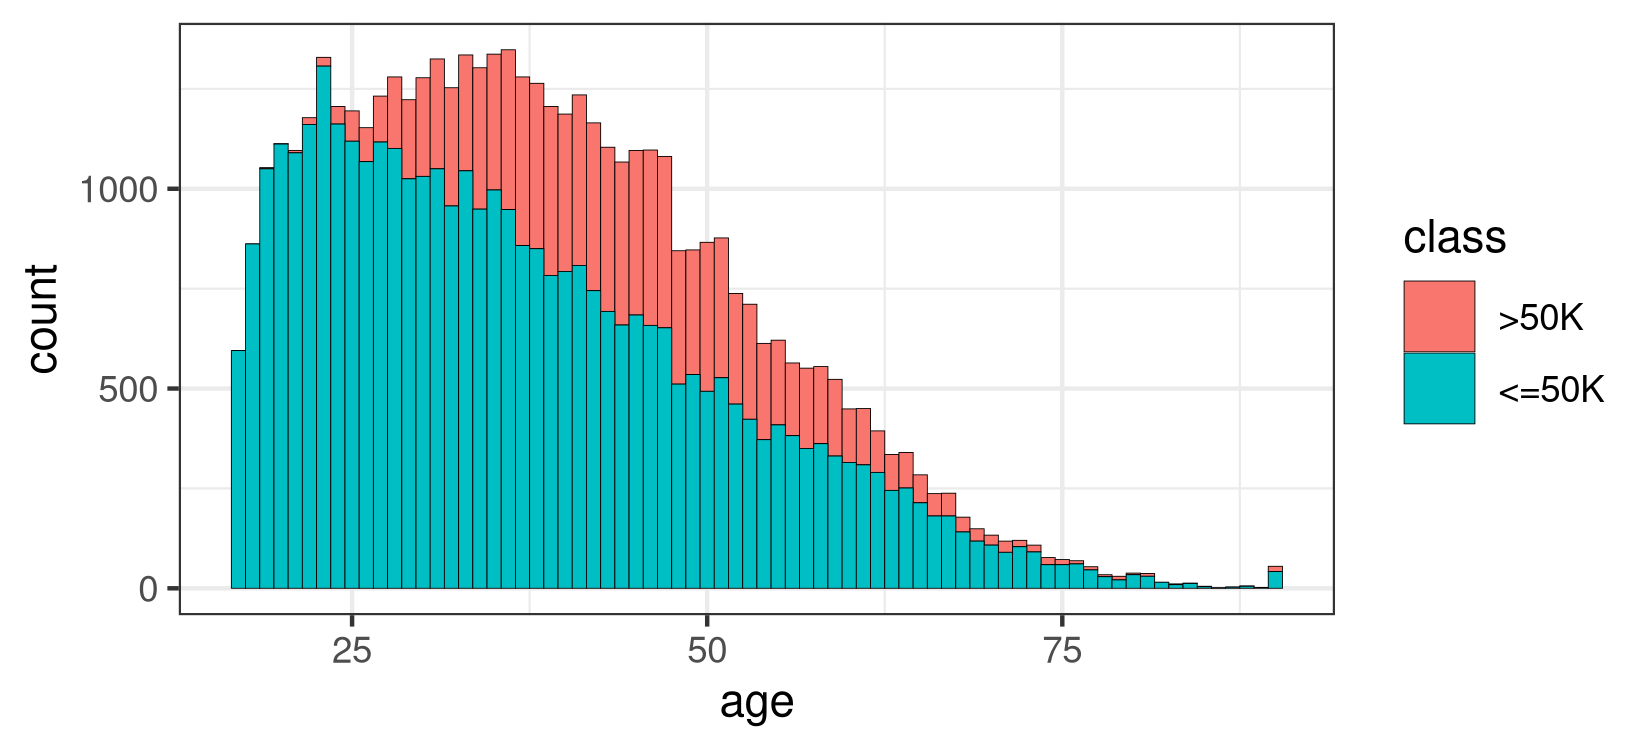
\includegraphics[scale = 0.45]{images/dataset_adult_age_sex.png}
\end{column}%
\begin{column}{0.6\textwidth}

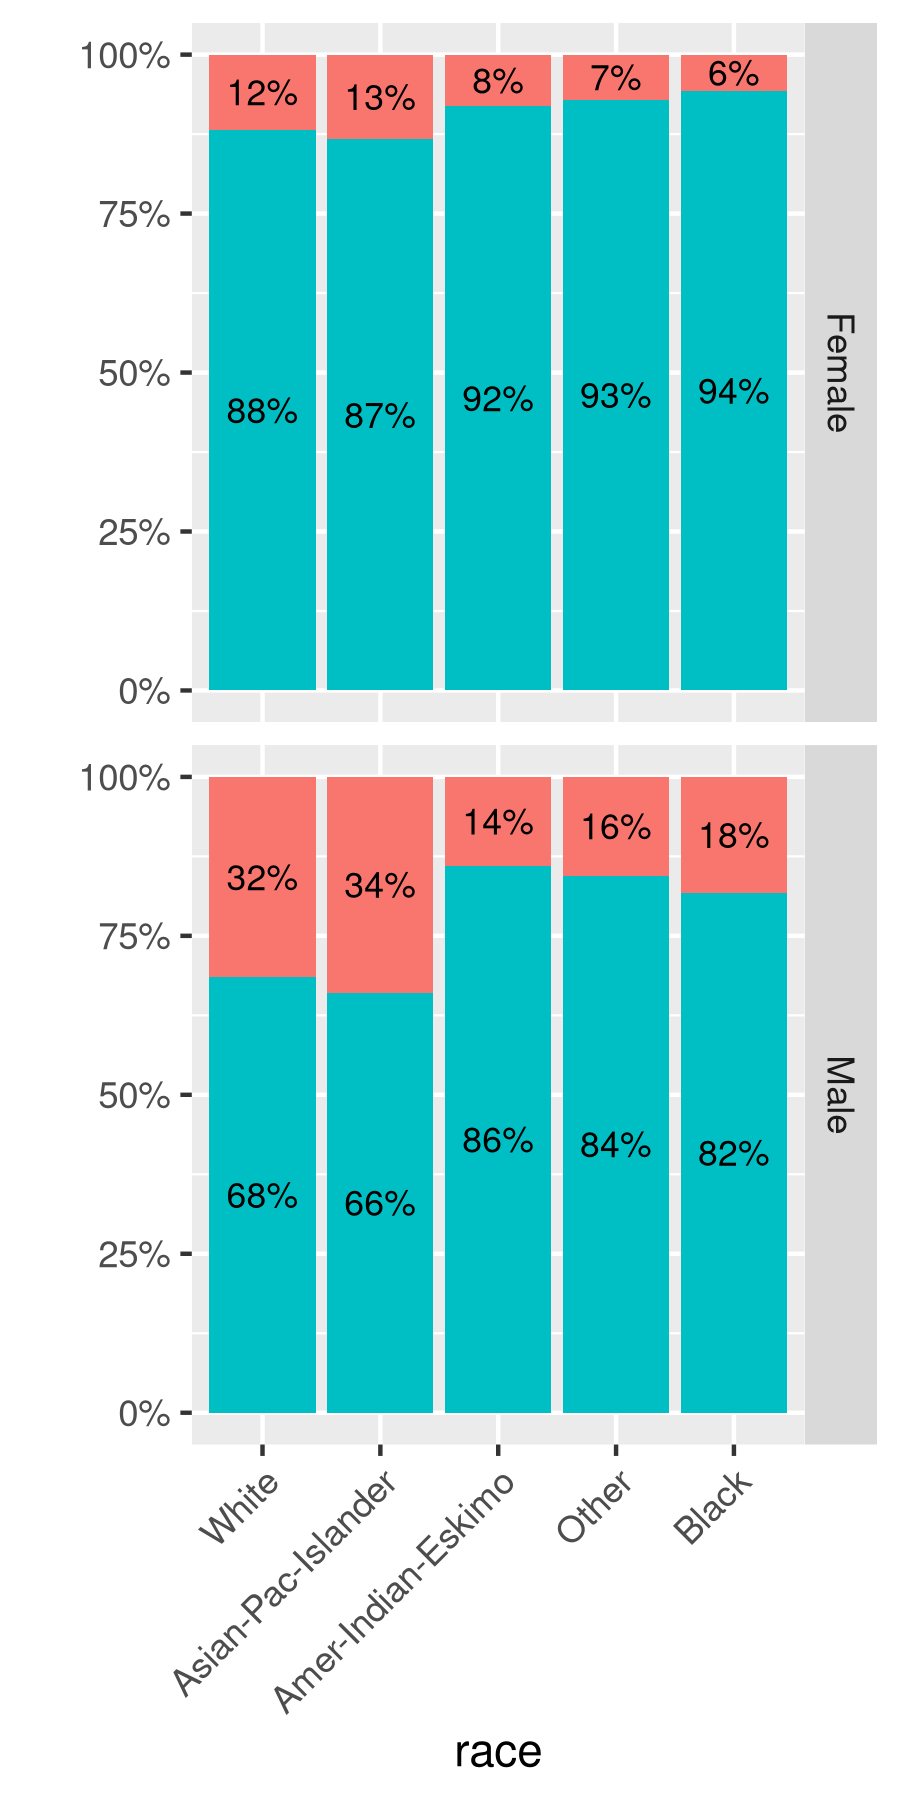
\includegraphics[scale = 0.45]{images/dataset_adult_race.png}%
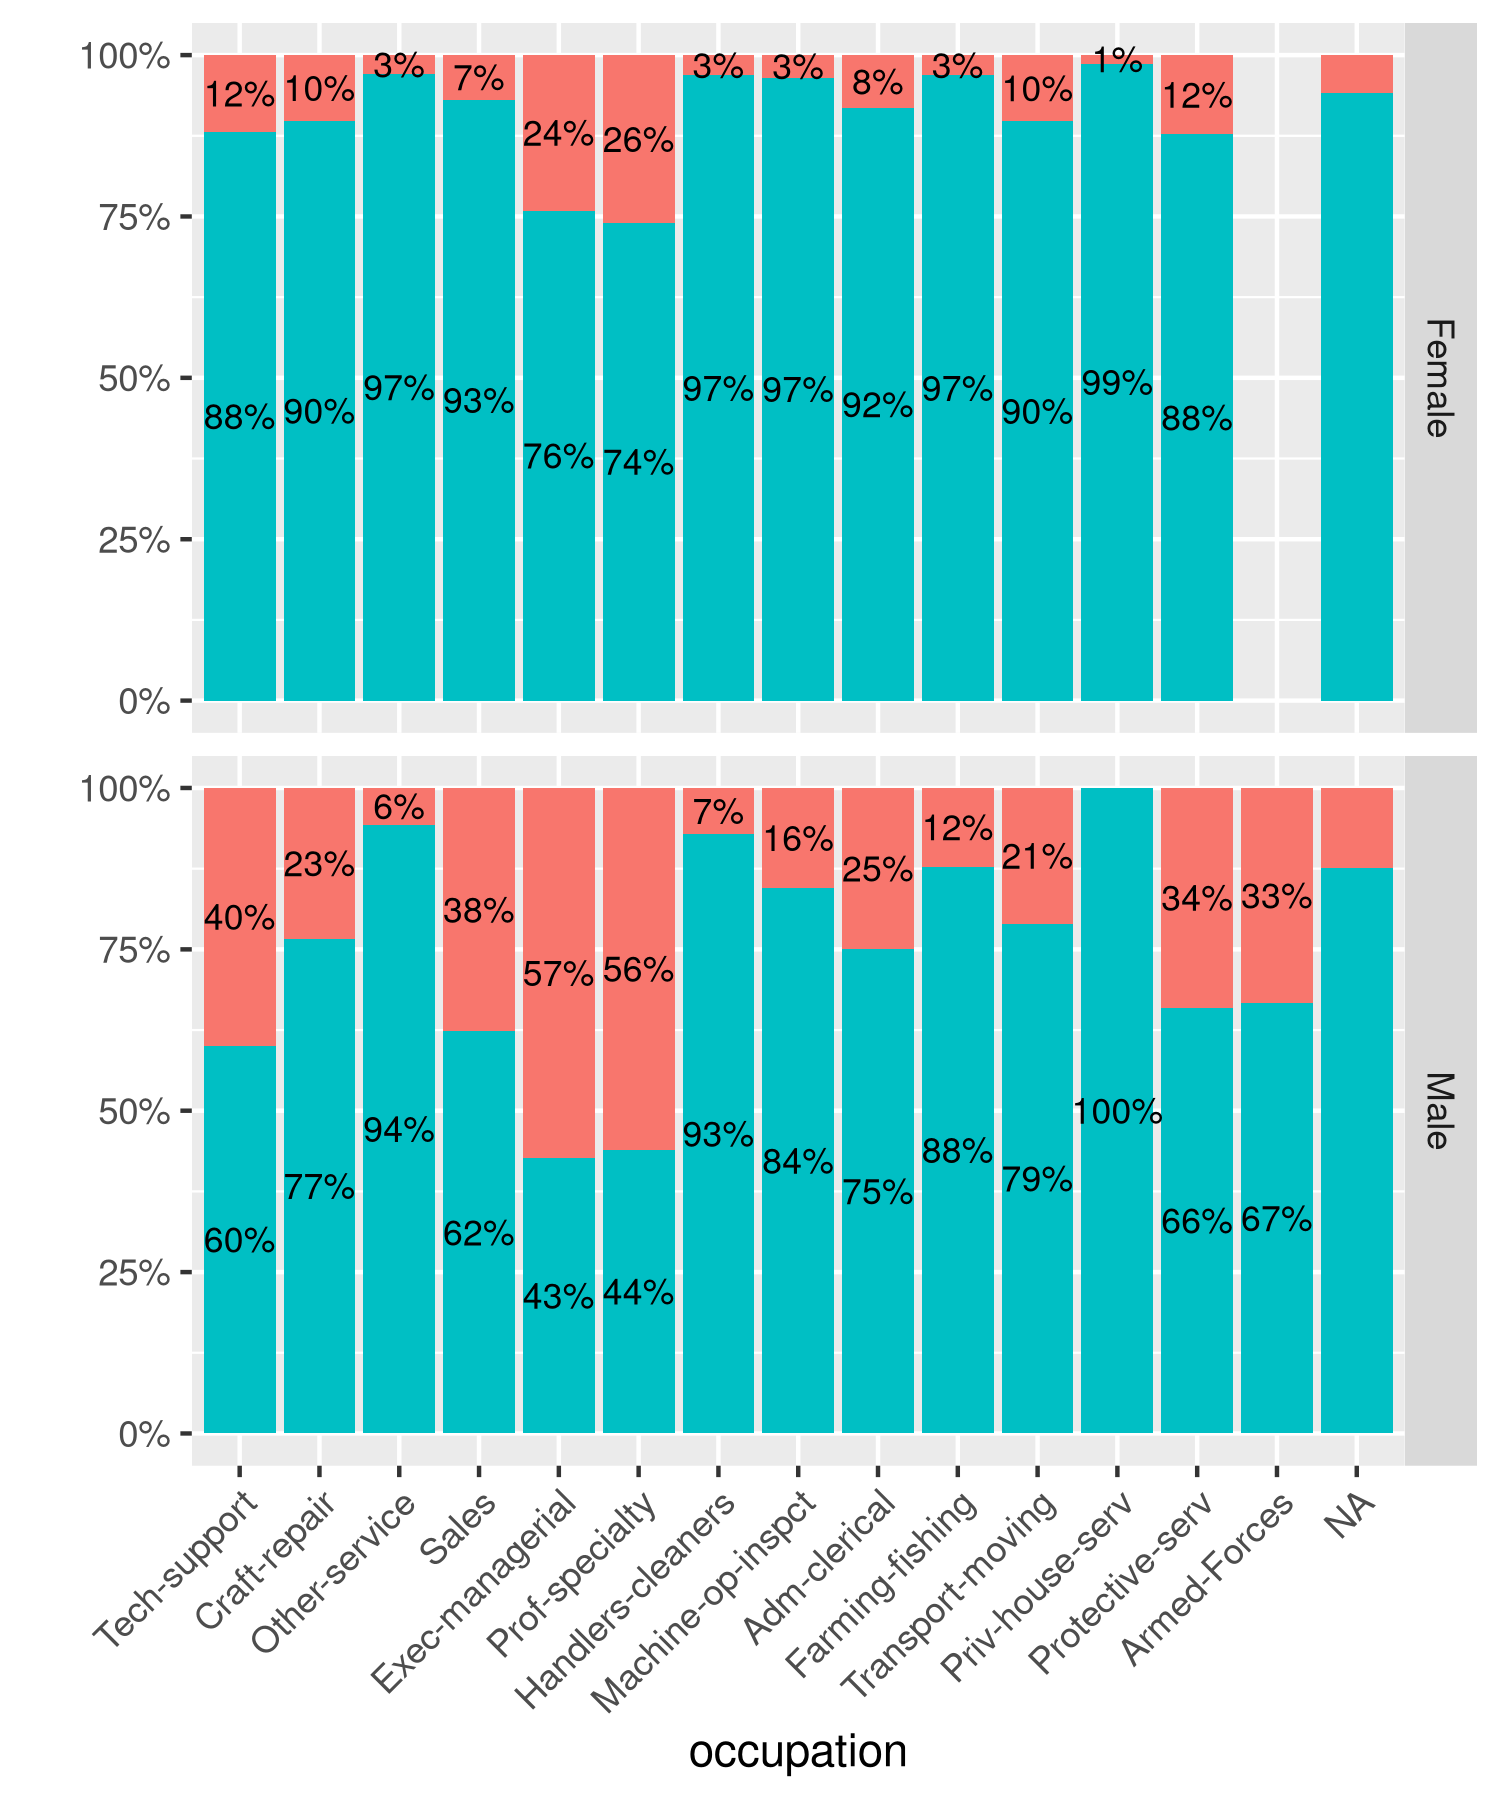
\includegraphics[scale = 0.45]{images/dataset_adult_education.png}
\end{column}
\end{columns}


\end{frame}

\begin{frame}[allowframebreaks]{Fair Models - Setup}
  A fair model for income prediction on binarized target.
%\begin{columns}
%\begin{column}{0.5\textwidth}
\begin{itemize}
  \item Learner: \emph{eXtreme Gradient Boosting}
  \item Hyperparameters to optimize: \\
  \begin{tabular}{rl}
    \texttt{eta} & $[0.01,0.2]$ \\
    \texttt{gamma} & $[2^{-7},2^6]$ \\
    \texttt{max\_depth} & $\{2, \ldots, 20\}$ \\
    \texttt{colsample\_bytree} & $[0.5,1]$ \\
    \texttt{colsample\_bylevel} & $[0.5,1]$ \\
    \texttt{lambda} & $[2^{-10},2^{10}]$ \\
    \texttt{alpha} & $[2^{-10},2^{10}]$ \\
    \texttt{subsample} & $[0.5,1]$ \\
  \end{tabular}
  \item Objective: minimize \emph{missclassification error} and \emph{fairness}
%\end{itemize}
%\end{column}%
%\begin{column}{0.5\textwidth}
%\begin{itemize}
  \item "Is the rate of classified as high income equal amongst both subgroups given the prevalence in each subgroup?"
  \item Here, a simplified proxy for fairness is defined as the absolute difference in F1-Scores between female ($f$) and male ($m$) population:
  \[
  \loss_{\text{fair}} := |\loss_{\text{F1}}(y_f,\fh(\x_f)) - \loss_{\text{F1}}(y_m,\fh(\x_m))|
  \]
  \item Optimizer: ParEGO with Random Forest surrogate and restricted range of projections to $[0.1, 0.9]$ (No interest in very unfair or bad configurations).
\end{itemize}
\vspace{1em}
Note on this example:
\begin{itemize}
  \item Here, the hyperparameters actually have an effect on the defined \emph{fairness measure}.
  \item However, this is often not the case or not enough to ensure a fair model.
\end{itemize}
%\end{column}
%\end{columns}

\end{frame}

\begin{frame}{Fair Models - Results}

  \begin{figure}
    \centering
    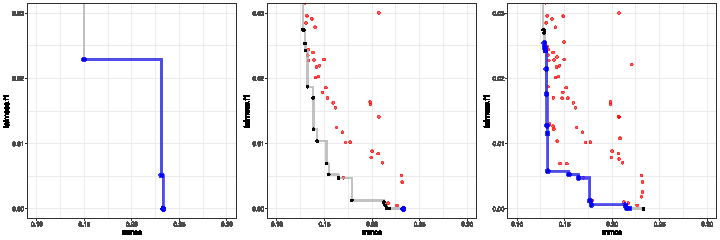
\includegraphics[scale=1.2]{images/Pfisterer_et_al_2019_Multi_Objective_fig4.pdf}
    \caption{Pareto fronts after 20, 70 and 120 tuning iterations.}
  \end{figure}

\end{frame}



\end{document}
